%==========================================================================

\begin{frame}[fragile]{}

  {\Huge Data parallel patterns}

  \vspace{20pt}

  \textbf{Learning objectives:}
  \begin{itemize}
    \item{How computational bodies are passed to the Kokkos runtime.}
    \item{How work is mapped to execution resources.}
    \item{The difference between \texttt{parallel\_for} and \texttt{parallel\_reduce}.}
    \item{Start parallelizing a simple example.}
  \end{itemize}

  \vspace{-20pt}

\end{frame}

%==========================================================================

\begin{frame}[fragile]{Using Kokkos for data parallel patterns (0)}

  \textbf{\ul{Data parallel patterns and work}}

  \begin{code}[linebackgroundcolor={
        \btLstHL<1->{2}{bodyColor}
      }
    ]
@patternfor@pattern (atomIndex = @policy0; atomIndex < numberOfAtoms; ++atomIndex@policy) {
  atomForces[atomIndex] = calculateForce(...data...);
}
  \end{code}

  Kokkos maps \textbf{work} to execution resources

  \pause

  \begin{itemize}
    \item {each iteration of a computational body is a \textbf{unit of work}.}
    \item {an \textbf{iteration index} identifies a particular unit of work.}
    \item {an \textbf{iteration range} identifies a total amount of work.}
  \end{itemize}

  \pause

  \vspace{0pt}

  \begin{block}{Important concept: Work mapping}
    You give an \textbf{iteration range} and \textbf{computational body} (kernel) \\
    to Kokkos, and Kokkos decides how to map that work to execution resources.
  \end{block}

  \vspace{-10pt}

\end{frame}

%==========================================================================

\begin{frame}[fragile]{Using Kokkos for data parallel patterns (2)}

  \textbf{How are computational bodies given to Kokkos?}

  \vspace{6pt}
  \pause

  \hspace{10pt} As \textbf{functors} or \textit{function objects}, a common pattern in C++.

  \pause
  \vspace{10pt}

  Quick review, a \textbf{functor} is a function with data. Example:
  \begin{code}[keywords={}, frame=single]
struct @darkredParallelFunctor@darkred {
  ...
  void operator()( <@\emph{a work assignment}@> ) const {
    @body/* ... computational body ... */@body
  ...
};
  \end{code}

\end{frame}

%==========================================================================

\begin{frame}[fragile]{Using Kokkos for data parallel patterns (3)}

  \textbf{How is work assigned to functor operators?}

  \vspace{6pt}
  \pause

  \hspace{10pt} A total amount of work items is given to a Kokkos pattern,
  \begin{code}[keywords={}, frame=single]
@darkredParallelFunctor@darkred @bluefunctor@blue;
@patternKokkos::parallel_for@pattern(@policynumberOfIterations@policy, @bluefunctor@blue);
  \end{code}

  \vspace{0pt}
  \pause

  \hspace{10pt} and work items are assigned to functors one-by-one:

  \begin{code}[keywords={}, frame=single]
@graystruct Functor {
  void operator()(@gray@blackconst int64_t index@black@gray) const {...}
}@gray
  \end{code}

  \pause
  \vspace{5pt}

  \begin{alertblock}{Warning: concurrency and order}
    Concurrency and ordering of parallel iterations is \textit{not} guaranteed by the Kokkos runtime.
  \end{alertblock}

  \vspace{0pt}

\end{frame}

%==========================================================================

\iffull
\begin{frame}[fragile]{Using Kokkos for data parallel patterns (4)}

  \textbf{How is data passed to computational bodies?}

  \vspace{2pt}

  \begin{code}
for (atomIndex = 0; atomIndex < numberOfAtoms; ++atomIndex) {
  @darkgreenatomForces@darkgreen[atomIndex] = calculateForce(@darkred...data...@darkred);
}
  \end{code}

  \vspace{-3pt}

  \begin{code}[keywords={}, frame=single]
@graystruct AtomForceFunctor {
  ...
  void operator()(const int64_t atomIndex) const {@gray
    @darkgreenatomForces@darkgreen[atomIndex] = calculateForce(@darkred...data...@darkred);
  @gray}
  ...
}@gray
  \end{code}
  \pause
  \vspace{5pt}

  How does the body access the data?

  \vspace{-3pt}

  \begin{block}{Important concept}
    A parallel functor body must have access to all the data it needs through the functor's \textbf{data members}.
  \end{block}

\end{frame}
\fi

%==========================================================================

\iffull
\begin{frame}[fragile]{Using Kokkos for data parallel patterns (5)}

  \textbf{\ul{Putting it all together: the complete functor}}:

  \begin{code}[keywords={}, frame=single]
struct AtomForceFunctor {
  <@\emph{ForceType}@> @darkgreen_atomForces;@darkgreen
  <@\emph{DataType}@> @darkred_atomData;@darkred
  AtomForceFunctor(/* args */) {...}
  void operator()(const int64_t atomIndex) const {
    @darkgreen_atomForces@darkgreen[atomIndex] = calculateForce(@darkred_atomData@darkred);
  }
};
  \end{code}

  \vspace{5pt}
  \pause

  \textbf{Q/} How would we \textbf{reproduce serial execution} with this functor?

  \vspace{3pt}

  \begin{code}[keywords={}, frame=single]
for (atomIndex = 0; atomIndex < numberOfAtoms; ++atomIndex){
  @darkgreenatomForces@darkgreen[atomIndex] = calculateForce(@darkreddata@darkred);
}
  \end{code}

  \begin{textblock*}{0.5\textwidth}(0.05\textwidth,0.600\textheight)
    \only<2->{\rotatebox{90}{\textbf{Serial}}}
  \end{textblock*}

  %\vspace{3pt}
  \pause

  \begin{code}[keywords={}, frame=single]
AtomForceFunctor @bluefunctor@blue(@darkgreenatomForces@darkgreen, @darkreddata@darkred);
for (atomIndex = 0; atomIndex < numberOfAtoms; ++atomIndex){
  @bluefunctor@blue(atomIndex);
}
  \end{code}

  \begin{textblock*}{0.5\textwidth}(0.05\textwidth,0.755\textheight)
    \only<3->{\rotatebox{90}{\textbf{Functor}}}
  \end{textblock*}

\end{frame}
\fi

%==========================================================================

\begin{frame}[fragile]{Using Kokkos for data parallel patterns (6)}

  \textbf{\ul{The complete picture}} (using functors):

  \vspace{8pt}

  1.  Defining the functor (operator+data):

  \vspace{0pt}

  \begin{code}[keywords={}, frame=single]
struct AtomForceFunctor {
  <@\emph{ForceType}@> @darkgreen_atomForces;@darkgreen
  <@\emph{DataType}@> @darkred_atomData;@darkred

  AtomForceFunctor(<@\emph{ForceType}@> atomForces, <@\emph{DataType}@> data) :
    @darkgreen_atomForces@darkgreen(atomForces), @darkred_atomData@darkred(data) {}

  void operator()(const int64_t atomIndex) const {
    @body@darkgreen_atomForces@darkgreen[atomIndex] = calculateForce(@darkred_atomData@darkred);@body
  }
}
  \end{code}

  \vspace{5pt}

  2.  \textbf{Executing} in parallel with Kokkos pattern:

  \vspace{-4pt}

  \begin{code}
AtomForceFunctor functor(atomForces, data);
@patternKokkos::parallel_for@pattern(@policynumberOfAtoms@policy, functor);
  \end{code}

\end{frame}

%==========================================================================

\begin{frame}[fragile]{Using Kokkos for data parallel patterns (7)}

  Functors are tedious $\Rightarrow$ \ul{\textbf{C++11 Lambdas} are concise}

  \vspace{5pt}

  \begin{code}[linebackgroundcolor={
        \btLstHL<1->{4-6}{black!15}
      },
      keywords={}, frame=single]
@grayatomForces already exists
data already exists
Kokkos::parallel_for(numberOfAtoms, @gray
    [=] (const int64_t atomIndex) {
    @darkgreenatomForces@darkgreen[atomIndex] = calculateForce(@darkreddata@darkred);
  }
@gray);@gray
  \end{code}

  \pause

  A lambda is not \textit{magic}, it is the compiler \textbf{auto-generating} a \textbf{functor} for you.

  \pause
  \vspace{7pt}

  \begin{alertblock}{Warning: Lambda capture and C++ containers}
    For portability to GPU a lambda must capture by value \texttt{[=]}. \\
    Don't capture containers (\textit{e.g.}, std::vector)
    by value because it will copy the container's entire contents.
  \end{alertblock}

  %\pause
  %$\Rightarrow$ So, {\color{darkgreen}\texttt{atomForces}} must be a pointer (e.g., not a \texttt{std::vector})

\end{frame}

%==========================================================================

\begin{frame}[fragile]{parallel\_for examples}

  \textbf{How does this compare to OpenMP?}

  \vspace{5pt}

  \begin{code}[linebackgroundcolor={
      },
      frame=single
    ]
for (int64_t i = 0; i < N; ++i) {
  /* loop body */
}
  \end{code}

  \begin{code}[linebackgroundcolor={
        \btLstHL<1->{3}{bodyColor}
      },
      frame=single
    ]
#pragma @policyomp parallel@policy @patternfor@pattern
@patternfor@pattern (int64_t i = @policy0; i < N@policy; ++i) {
  /* loop body */
}
  \end{code}

  \begin{code}[linebackgroundcolor={
        \btLstHL<1->{2}{bodyColor}
      },
      frame=single
    ]
@patternparallel_for@pattern(@policyN@policy, [=] (const int64_t i) {
  /* loop body */
});
  \end{code}


  \begin{textblock*}{0.5\textwidth}(0.05\textwidth,0.200\textheight)
    \rotatebox{90}{\textbf{Serial}}
  \end{textblock*}

  \begin{textblock*}{0.5\textwidth}(0.05\textwidth,0.350\textheight)
    \rotatebox{90}{\textbf{OpenMP}}
  \end{textblock*}

  \begin{textblock*}{0.5\textwidth}(0.05\textwidth,0.550\textheight)
    \rotatebox{90}{\textbf{Kokkos}}
  \end{textblock*}


  \begin{block}{Important concept}
    Simple Kokkos usage is \textbf{no more conceptually difficult} than OpenMP, the annotations just go in different places.
  \end{block}

\end{frame}

%==========================================================================

\begin{frame}[fragile]{Scalar integration (0)}

  \textbf{\ul{Riemann-sum-style numerical integration}}:

  \vspace{-20pt}

  \begin{columns}[t,onlytextwidth]
    \column{.50\textwidth}
      \vspace{10pt}
      \[y = \int_{\textcolor{darkred}{lower}}^{\textcolor{blue}{upper}} {\textcolor{darkgreen}{function}}(x)\,dx\]
    \column{.50\textwidth}
      \begin{center}
      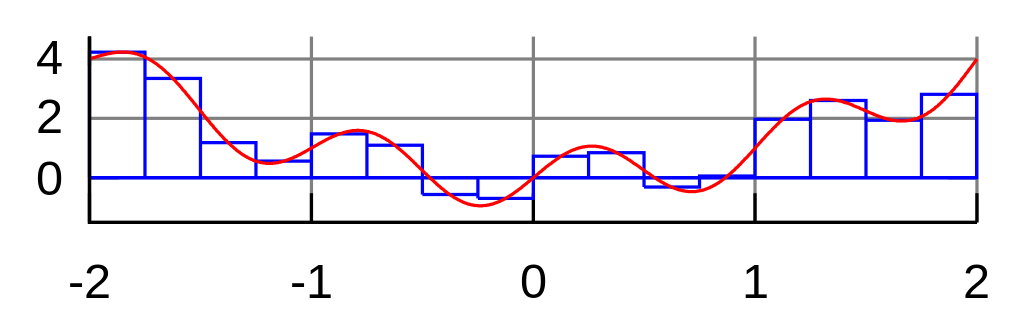
\includegraphics[width=1.0\textwidth]{figures/NumericalIntegration_rectangle}
      \end{center}
      \vspace{-22pt}
      \hspace*{15pt}\hbox{\thinspace{\tinytiny\itshape Wikipedia}}
  \end{columns}

  \vspace{15pt}
  \pause

  \begin{onlyenv}<1>
    \vspace{89pt}
  \end{onlyenv}

  \begin{onlyenv}<2-3>
  \begin{code}[linebackgroundcolor={
      }
    ]
double totalIntegral = 0;
for (int64_t i = 0; i < numberOfIntervals; ++i) {
  const double @orangex@orange =
    <@${\textcolor{darkred}{lower}}$@> + (i/numberOfIntervals) * (<@${\textcolor{blue}{upper}}$@> - <@${\textcolor{darkred}{lower}}$@>);
  const double thisIntervalsContribution = <@${\textcolor{darkgreen}{function}}$@>(@orangex@orange);
  totalIntegral += thisIntervalsContribution;
}
totalIntegral *= dx;
  \end{code}
  \end{onlyenv}

  \begin{onlyenv}<1-3>
    \vspace{10pt}
  \end{onlyenv}

  \begin{onlyenv}<4->
  \begin{code}[linebackgroundcolor={
        \btLstHL<4->{3-6}{bodyColor}
      }
    ]
double totalIntegral = 0;
@patternfor@pattern (int64_t @policyi = 0; i < numberOfIntervals; ++i@policy) {
  const double @orangex@orange =
    <@${\textcolor{darkred}{lower}}$@> + (i/numberOfIntervals) * (<@${\textcolor{blue}{upper}}$@> - <@${\textcolor{darkred}{lower}}$@>);
  const double thisIntervalsContribution = <@${\textcolor{darkgreen}{function}}$@>(@orangex@orange);
  totalIntegral += thisIntervalsContribution;
}
totalIntegral *= dx;
  \end{code}

  \begin{textblock*}{0.5\textwidth}(0.09\textwidth,0.45\textheight)
    \only<4->{\footnotesize {\color{orange!80} Pattern?}}
  \end{textblock*}

  \begin{textblock*}{0.5\textwidth}(0.76\textwidth,0.49\textheight)
    \only<4->{\footnotesize {\color{darkgreen!80} Policy?}}
  \end{textblock*}

  \begin{textblock*}{0.5\textwidth}(0.08\textwidth,0.585\textheight)
    \only<4->{\rotatebox{90}{\footnotesize {\color{blue!80} Body?}}}
  \end{textblock*}
  \pause
  \vspace{10pt}

  \end{onlyenv}

  \begin{onlyenv}<1-2>
    \vspace{10pt}
  \end{onlyenv}

  \begin{onlyenv}<3-4>
  How do we \textbf{parallelize} it?  \textit{Correctly?}
  \end{onlyenv}

\end{frame}

%==========================================================================

\begin{frame}[fragile]{Scalar integration (1)}

  \textbf{\ul{An (incorrect) attempt}}:

  \vspace{5pt}

  \begin{code}[linebackgroundcolor={
        \btLstHL<1->{4-6}{bodyColor}
      },
      frame=single
    ]
double totalIntegral = 0;
@patternKokkos::parallel_for@pattern(@policynumberOfIntervals@policy,
  [=] (const int64_t index) {
    const double x =
      lower + (index/numberOfIntervals) * (upper - lower);
    totalIntegral += function(x);}
  );
totalIntegral *= dx;
  \end{code}

\vspace{15pt}

{\color{red}First problem}: compiler error; cannot increment \texttt{totalIntegral} \\
  \hspace{20pt}(lambdas capture by value and are treated as const!)

\end{frame}

%==========================================================================

\begin{frame}[fragile]{Scalar integration (2)}

  \textbf{\ul{An (incorrect) solution to the (incorrect) attempt}}:

  \vspace{5pt}

  \begin{code}[linebackgroundcolor={
      },
      frame=single
    ]
@graydouble totalIntegral = 0;@gray
@darkreddouble * totalIntegralPointer = &totalIntegral;@darkred
@grayKokkos::parallel_for(numberOfIntervals,
  [=] (const int64_t index) {
    const double x =
      lower + (index/numberOfIntervals) * (upper - lower);@gray
    @darkred*totalIntegralPointer@darkred @gray+= function(x);}
  );
totalIntegral *= dx;@gray
  \end{code}

  \pause
  \vspace{5pt}

  {\color{red}Second problem}: race condition

  \vspace{-7pt}

  \begin{center}
  \begin{tabular}{| c | c | c |}
    \hline
    step & thread 0 & thread 1 \\
    \hline
    0 & load & \\
    \hline
    1 & increment & load \\
    \hline
    2 & write & increment \\
    \hline
    3 & & write \\
    \hline
  \end{tabular}
  \end{center}

  \vspace{-7pt}

\end{frame}

%==========================================================================

\begin{frame}[fragile]{Scalar integration (3)}

  {\color{red}Root problem}: we're using the \textbf{wrong pattern}, \emph{for} instead of \emph{reduction}

  \pause
  \vspace{5pt}

  \begin{block}{Important concept: Reduction}
    Reductions combine the results contributed by parallel work.
  \end{block}

  \vspace{10pt}
  \pause

  How would we do this with \textbf{OpenMP}?

  \vspace{-3pt}

  \begin{code}[linebackgroundcolor={
        \btLstHL<3->{4}{bodyColor}
      }
    ]
double finalReducedValue = 0;
#pragma @policyomp parallel@policy @patternfor reduction@pattern(@pattern+:finalReducedValue@pattern)
@patternfor@pattern (int64_t i = @policy0; i < N; ++i@policy) {
  finalReducedValue += ...
}
  \end{code}

  \pause
  How will we do this with \textbf{Kokkos}?

  \vspace{-3pt}

  \begin{code}[linebackgroundcolor={
        \btLstHL<4->{4}{bodyColor}
      }
    ]
double finalReducedValue = 0;
@patternparallel_reduce@pattern(@policyN@policy, @bodyfunctor@body, finalReducedValue);
  \end{code}

  \vspace{-5pt}

\end{frame}

%==========================================================================

\begin{frame}[fragile]{Scalar integration (4)}

  \ul{\textbf{Example: Scalar integration}}

  \vspace{5pt}

  \begin{code}[linebackgroundcolor={
        \btLstHL<1->{4}{bodyColor}
      },
      frame=single
    ]
double totalIntegral;
#pragma @policyomp parallel@policy @patternfor reduction@pattern(@pattern+:totalIntegral@pattern)
@patternfor@pattern (int64_t i = @policy0; i < numberOfIntervals; ++i@policy) {
  totalIntegral += function(...);
}
  \end{code}

  \begin{code}[linebackgroundcolor={
        \btLstHL<1->{4}{bodyColor}
      },
      frame=single
    ]
double totalIntegral = 0;
@patternparallel_reduce@pattern(@policynumberOfIntervals@policy,
  [=] (const int64_t i, double & valueToUpdate) {
    valueToUpdate += function(...);
  },
  totalIntegral);
  \end{code}

  \begin{textblock*}{0.5\textwidth}(0.05\textwidth,0.22\textheight)
    \rotatebox{90}{\textbf{OpenMP}}
  \end{textblock*}

  \begin{textblock*}{0.5\textwidth}(0.05\textwidth,0.49\textheight)
    \rotatebox{90}{\textbf{Kokkos}}
  \end{textblock*}

  \vspace{-5pt}

  \begin{itemize}
  \item The operator takes \textbf{two arguments}: a work index and a
  value to update.
  \item The second argument is a \textbf{thread-private value} that is
  managed by Kokkos; it is not the final reduced value.
    %by the way, that's what openmp is doing
  \end{itemize}

\end{frame}

%==========================================================================

\iffull
\begin{frame}[fragile]{Amdahl's Law (1)}

  \vspace{-10pt}
  \begin{alertblock}{Warning: Parallelism is NOT free}
    Dispatching (launching) parallel work has non-negligible cost.
  \end{alertblock}

  \pause

  {Simplistic data-parallel performance model: Time = $ \alpha + \frac{\beta * N}{P} $}
  \begin{itemize}
  \item {$\alpha$ = dispatch overhead}
  \item {$\beta$ = time for a unit of work}
  \item {$N$ = number of units of work}
  \item {$P$ = available concurrency}
  \end{itemize}

  \pause

  Speedup = {$P \div {\left( 1 + \frac{\alpha * P}{\beta * N} \right)}$}
  \begin{itemize}
  \item Should have {$\alpha * P \ll \beta * N$}
  \item \textit{All} runtimes strive to minimize launch overhead $\alpha$
  \item Find more parallelism to increase $N$
  \item Merge (fuse) parallel operations to increase $\beta$
  \end{itemize}

  \vspace{-10pt}

\end{frame}
\fi

%==========================================================================

\iffull
\begin{frame}[fragile]{Amdahl's Law (2)}

  \vspace{12pt}

  \textbf{\ul{Results}}:
  {illustrates simple speedup model = {$P \div {\left( 1 + \frac{\alpha * P}{\beta * N} \right)}$}}

  \vspace{-32pt}

  \begin{center}
    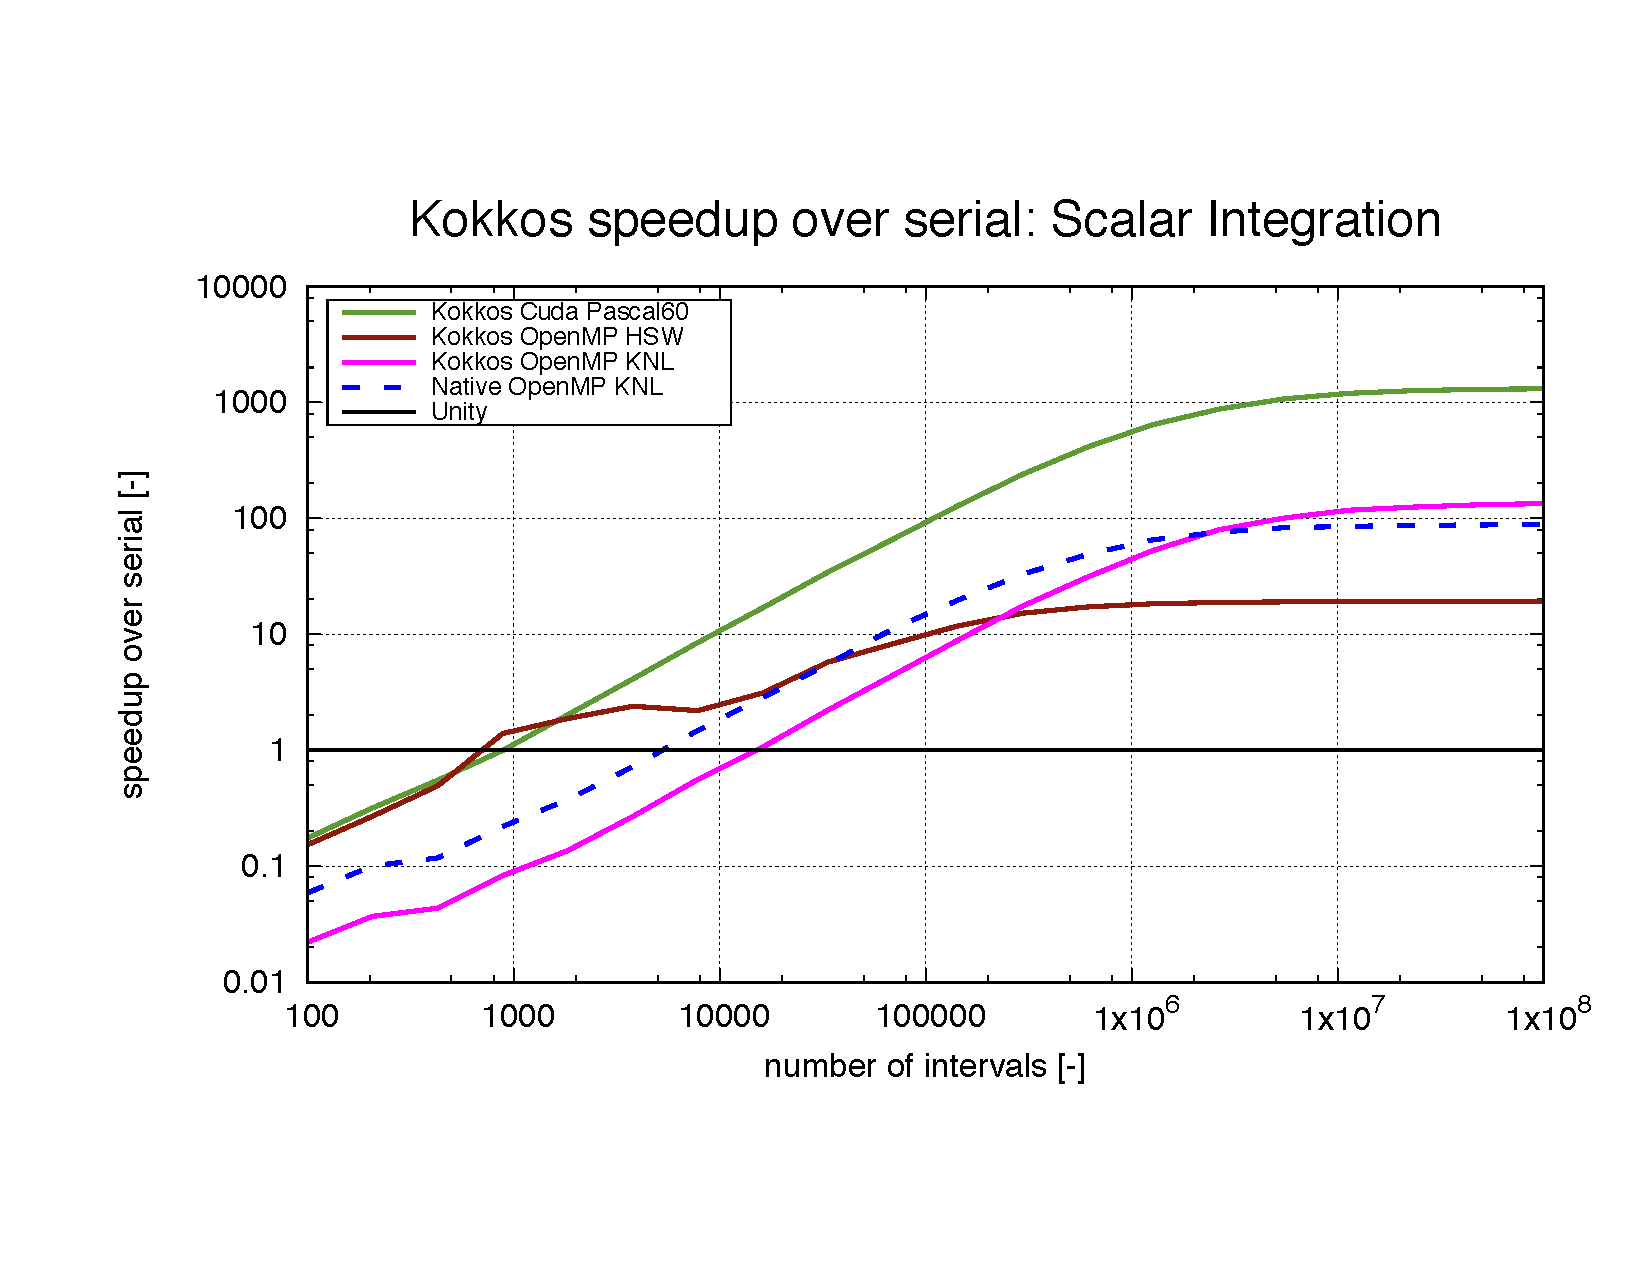
\includegraphics[width=1.00\textwidth]{figures/ScalarIntegration.pdf}
  \end{center}

  \vspace{-24pt}

  \begin{textblock*}{0.5\textwidth}(1.06\textwidth,0.33\textheight)
    \rotatebox{90}{\textbf{Note: log scale}}
  \end{textblock*}

\end{frame}
\fi

%==========================================================================

\begin{frame}[fragile]{Naming your kernels}
  \vspace{-10pt}
  \begin{alertblock}{Always name your kernels!}
     Giving unique names to each kernel is immensely helpful for debugging and profiling. You will regret it if you don't!
  \end{alertblock}
 
  \begin{itemize}
     \item Non-nested parallel patterns can take an optional string argument.
     \item The label doesn't need to be unique, but it is helpful.
     \item Anything convertible to "std::string"
     \item Used by profiling and debugging tools (see Profiling Tutorial)
  \end{itemize}
  \textbf{Example:} 
  \begin{code}[linebackgroundcolor={
        \btLstHL<1->{4}{bodyColor}
      },
      frame=single
    ]
double totalIntegral = 0;
@patternparallel_reduce@pattern("Reduction",@policynumberOfIntervals@policy,
  [=] (const int64_t i, double & valueToUpdate) {
    valueToUpdate += function(...);
  },
  totalIntegral);
  \end{code}
\end{frame}

%==========================================================================

\begin{frame}[fragile]{Recurring Exercise: Inner Product}

  \textbf{Exercise}: Inner product $<y, A * x>$

  \vspace{-10pt}

  \begin{center}
    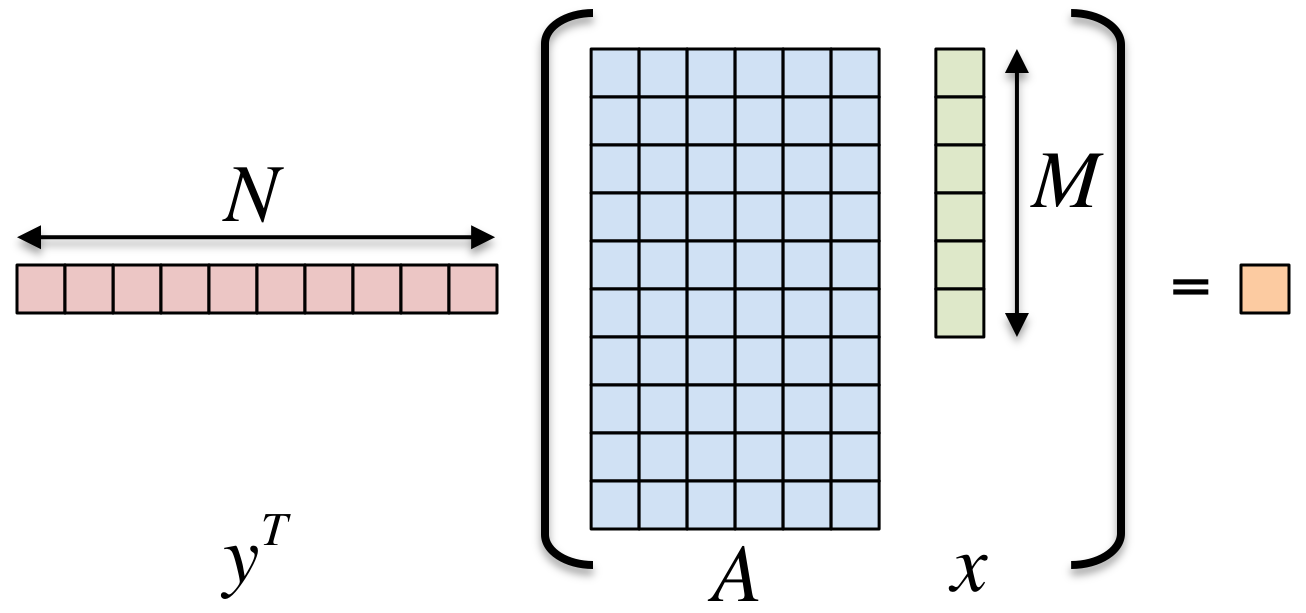
\includegraphics[width=0.80\textwidth]{figures/InnerProductExample_annotated}
  \end{center}

  \vspace{-15pt}

  \textbf{Details}:
  \begin{itemize}
    \item $y$ is $Nx1$, $A$ is $NxM$, $x$ is $Mx1$
    \item We'll use this exercise throughout the tutorial
  \end{itemize}

\end{frame}

%==========================================================================

\begin{frame}[fragile]{Exercise \#1: include, initialize, finalize Kokkos}

  The \textbf{first step} in using Kokkos is to include, initialize, and finalize:

  \begin{code}
#include <Kokkos_Core.hpp>
int main(int argc, char* argv[]) {
  /* ... do any necessary setup (e.g., initialize MPI) ... */
  Kokkos::initialize(argc, argv);
  {
  /* ... do computations ... */
  }
  Kokkos::finalize();
  return 0;
}
  \end{code}

  \vspace{7pt}

  (Optional) Command-line arguments or environment variables:

  \vspace{3pt}

	\begin{tabular}{| p{0.5\textwidth} | p{0.5\textwidth} |}
    \hline
	  \texttt{--kokkos-num-threads=INT} or \texttt{KOKKOS\_NUM\_THREADS} & total number of threads \\
    \hline
	  \texttt{--kokkos-device-id=INT} or \texttt{KOKKOS\_DEVICE\_ID} & device (GPU) ID to use \\
    \hline
  \end{tabular}

\end{frame}

%==========================================================================


\begin{frame}[fragile]{Exercise \#1: Inner Product, Flat Parallelism on the CPU}

  \vspace{5pt}

  \textbf{Exercise}: Inner product $<y, A * x>$

  \vspace{-10pt}

  \begin{center}
    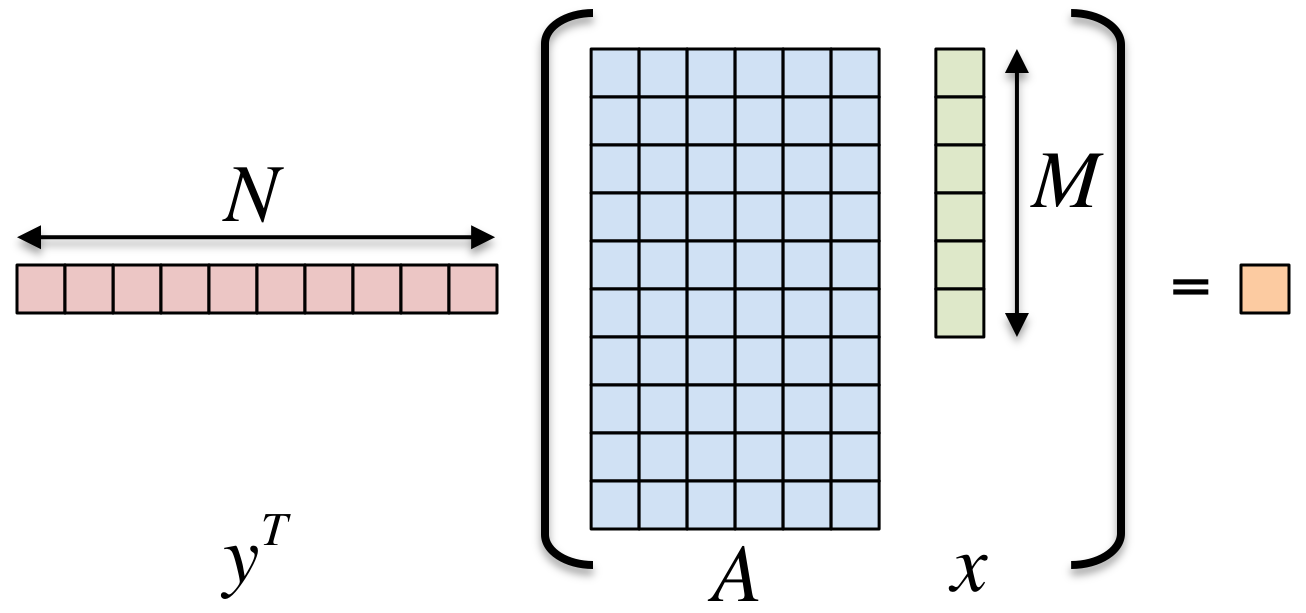
\includegraphics[width=0.65\textwidth]{figures/InnerProductExample_annotated}
  \end{center}

  \vspace{-30pt}

  \textbf{Details}:
  \begin{small}
  \begin{itemize}
\item Location: \ExerciseDirectory{01/Begin}
\item Look for comments labeled with ``EXERCISE''
\item Need to include, initialize, and finalize Kokkos library
\item Parallelize loops with \texttt{parallel\_for} or \texttt{parallel\_reduce}
\item Use lambdas instead of functors for computational bodies.
\item For now, this will only use the CPU.
\end{itemize}
  \end{small}

\end{frame}

%==========================================================================

\begin{frame}[fragile]{Exercise \#1: logistics}

\ul{\textbf{Compiling for CPU}}

\vspace{-3pt}
  \begin{small}
  \begin{code}
  cmake -B build_openmp -DKokkos_ENABLE_OPENMP=ON \
      -DCMAKE_BUILD_TYPE=Release
  cmake --build build_openmp
  \end{code}
  \end{small}

%  \hspace{10pt} {\tiny \url{https://github.com/kokkos/kokkos/wiki/Compiling#table-43-architecture-variables}}

\ul{\textbf{Running on CPU} with OpenMP backend}

\vspace{-3pt}
  \begin{small}
  \begin{code}
  # Set OpenMP affinity
  export OMP_NUM_THREADS=8
  export OMP_PROC_BIND=spread OMP_PLACES=threads
  # Print example command line options:
  ./build_openmp/01_Exercise -h
  # Run with defaults on CPU
  ./build_openmp/01_Exercise
  # Run larger problem
  ./build_openmp/01_Exercise -S 26
  \end{code}
  \end{small}

\ul{\textbf{Things to try:}}
  \begin{small}
  \begin{itemize}
  \itemsep0em
%  \item Vary number of threads
  \item Vary problem size with command line argument -S $s$
  \item Vary number of rows with command line argument -N $n$
  \item Num rows = $2^n$, num cols = $2^m$, total size = $2^s == 2^{n+m}$
  \end{itemize}
  \end{small}
\end{frame}

%==========================================================================

\begin{frame}[fragile]{Exercise \#1 results}

  \vspace{-10pt}

  \begin{center}
    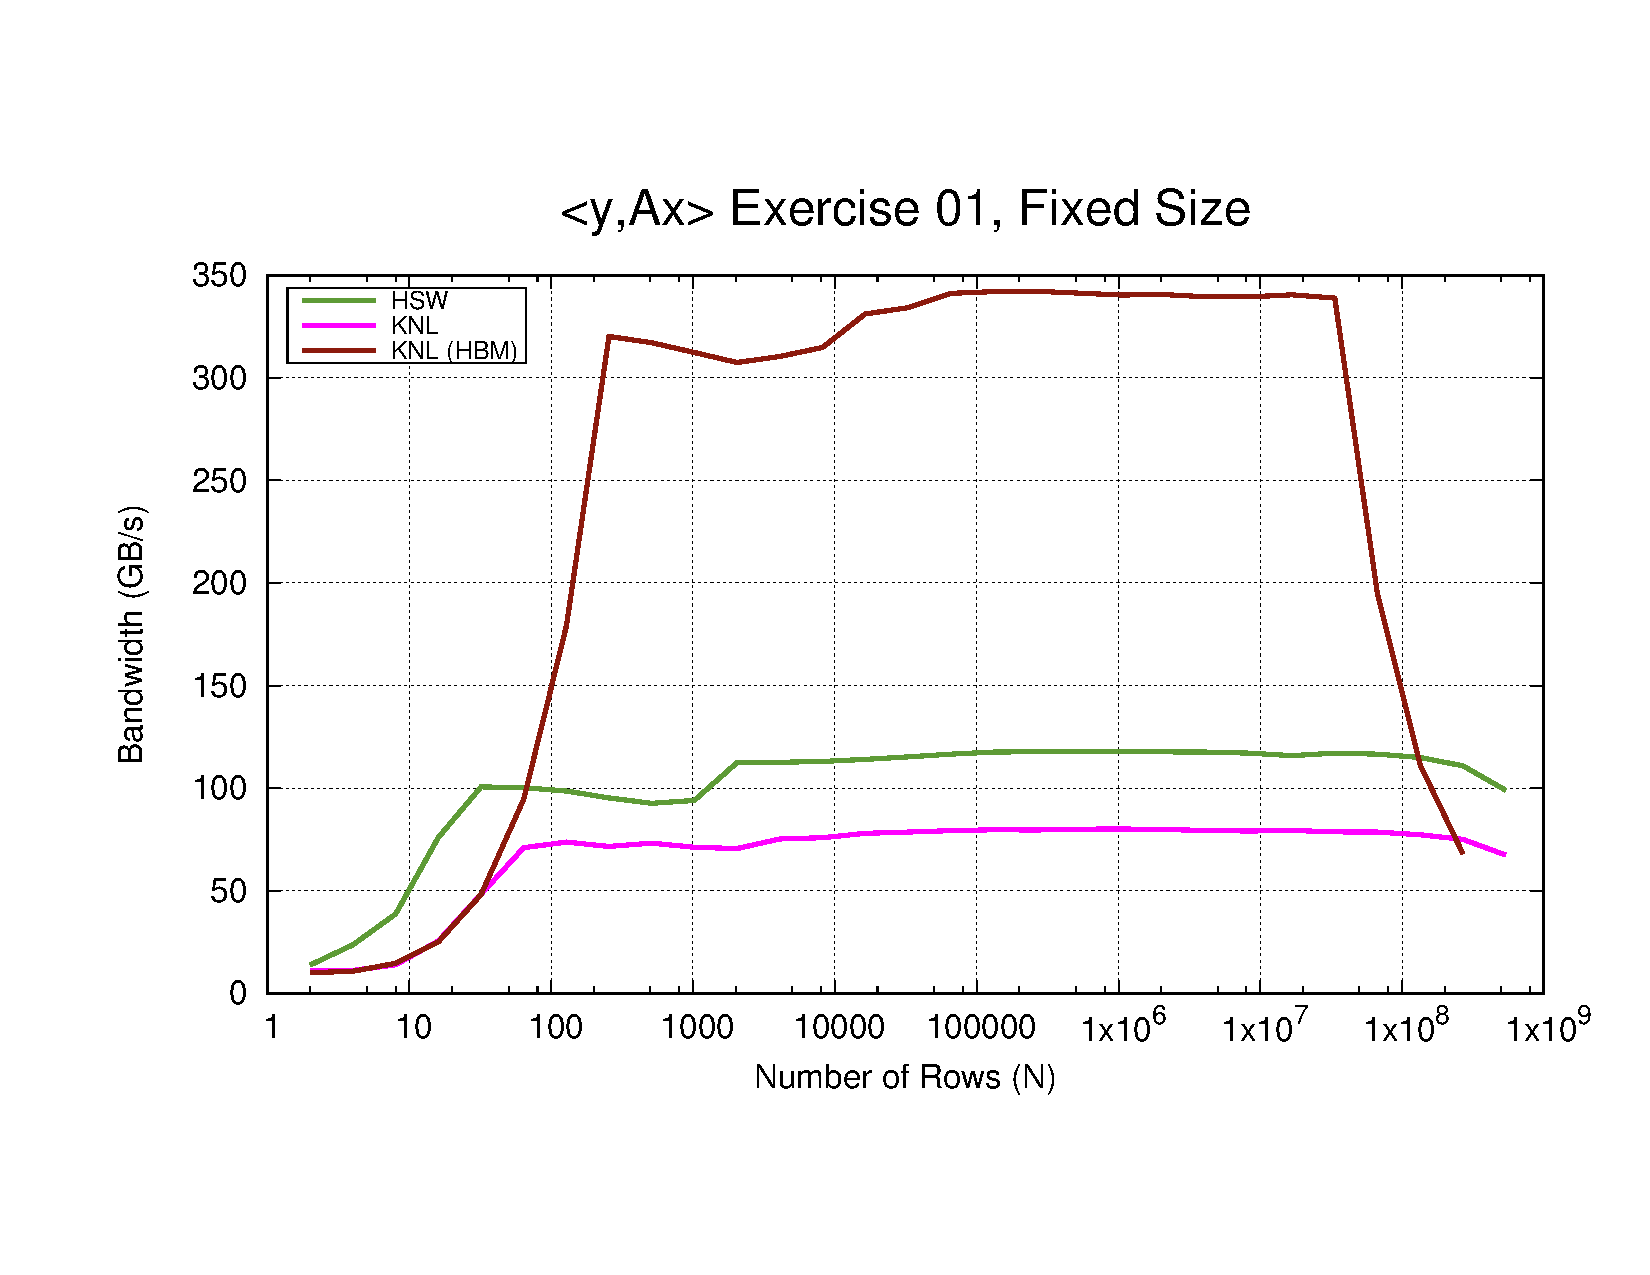
\includegraphics[viewport=1.25in 3.0in 10in 6in, width=1.0\textwidth]{figures/Exercise01-Performance.pdf}
  \end{center}

  \vspace{-15pt}

\end{frame}

%==========================================================================

\iffull
\begin{frame}[fragile]{Exercise \#1 Going beyond}
   \ul{\textbf{More things to try: port your solution to work on the device}}
   \begin{itemize}
     \item You will need to update the dynamic memory allocation.
     \item Replace \texttt{std::malloc} and \texttt{std::free} with \texttt{Kokkos::kokkos\_malloc} and \texttt{Kokkos::kokkos\_free}.
     \item Bonus question:  Why does this perform so poorly?  (hint: the answer is in this slide deck somewhere)
     \item Note that this is just for learning purposes and by no mean a recommended way to manage the lifetime of your arrays.  We will see a better way to do this soon.
   \end{itemize}

   \ul{\textbf{Compiling for GPU}}
  \vspace{-3pt}
  \begin{small}
  \begin{code}
  # if the architecture autodetection fails configure with
  # -DKokkos_ARCH_VOLTA70=ON for V100
  # refer to the documentation for the complete list of supported NVIDIA GPU
  # architectures and corresponding flags, or use ccmake to discover options
    cmake -B build-cuda -DKokkos_ENABLE_CUDA=ON
    cmake --build build-cuda
    make -j KOKKOS_DEVICES=Cuda KOKKOS_ARCH=...
  \end{code}
  \end{small}
\end{frame}
\fi

%==========================================================================

\iffull
\begin{frame}[fragile]{Basic capabilities we haven't covered}

  \begin{itemize}

  \item {Customizing \texttt{parallel\_reduce} data type and reduction operator
    \\ \hspace{10pt} \emph{e.g.}, minimum, maximum, ...}

  \item {\texttt{parallel\_scan} pattern for exclusive and inclusive prefix sum}

  \item {Using \textit{tag dispatch} interface to allow non-trivial functors to have multiple ``\texttt{operator()}'' functions.
    \\ \hspace{10pt} very useful in large, complex applications}

  \end{itemize}

\end{frame}
\fi

%==========================================================================

\begin{frame}{Section Summary}

  \begin{itemize}
    \item{\textbf{Simple} usage is similar to OpenMP, advanced features are also straightforward}
    \item{Three common \textbf{data-parallel patterns} are \texttt{parallel\_for}, \texttt{parallel\_reduce}, and \texttt{parallel\_scan}.}
    \item{A parallel computation is characterized by its \textbf{pattern}, \textbf{policy}, and \textbf{body}.}
    \item{User provides \textbf{computational bodies} as functors or lambdas which handle a single work item.}
  \end{itemize}

\end{frame}
